\section{问题分析与总体框架}\label{sec:analysis}

\subsection{目标函数的精确形式}

按\cref{asu:time}，把一局任务中的全部动作按类型归并，整局虚拟总时间可以写成一个精确的线性表达式：
\begin{equation}\label{eq:objective}
  T \;=\; \underbrace{\frac{L}{v}}_{\text{移动}}
        \;+\; \underbrace{t_m N_m}_{\text{检测}}
        \;+\; \underbrace{t_s N_s}_{\text{切频}}
        \;+\; \underbrace{t_f N_f}_{\text{光学失败}}
        \;+\; \underbrace{t_c N_c}_{\text{成功清除}}
  \;=\; \frac{L}{5}+5N_m+N_s+3N_f+5N_c .
\end{equation}
这里 $t_c=5\msec$ 已经包含了成功那一次的光学精确定位 $3\msec$ 与激光清除 $2\msec$，计算时只计一次。题目要求的两个统计量是
\begin{equation}\label{eq:metric}
  \text{清除比例}=\frac{N_c}{n},\qquad
  \bar T=\frac{T}{N_c},
\end{equation}
其中 $n$ 为该局真实源数。于是优化问题为
\begin{equation}\label{eq:opt}
  \min_{\pi}\ \mathbb E\!\left[T(\pi)\right]
  \quad\text{s.t.}\quad N_c(\pi)=n\ \text{以概率 }1,
\end{equation}
$\pi$ 是一个只依赖历史观测的在线策略（\cref{asu:info}）。本文把约束收紧为“以概率 $1$”，这是所有布局设计的出发点：以清除率 $100\%$ 为硬约束、以时间为优化目标，覆盖保证优先（该取舍的定量代价在\cref{sec:eval}中另行讨论）。

\paragraph{两种平均口径，全文一律标注.} 一批 $M$ 局测试有两种求平均的方式，它们是不同的量：
\begin{equation}\label{eq:twomeans}
  \bar T_{\text{案例}}=\frac1M\sum_{i=1}^{M}\frac{T_i}{N_i},
  \qquad
  \bar T_{\text{合并}}=\frac{\sum_i T_i}{\sum_i N_i}.
\end{equation}
前者每局等权，回答“随机抽一局的平均每源耗时是多少”；后者按源数加权，回答“累计处理每个源的总体成本是多少”。源多的局 $\bar T$ 偏小，所以合并口径通常略低于案例口径。两种口径各有用途，但比较两个版本时必须用同一口径。本文所有表格均在表题或表注中注明采用哪一种，跨表引用数字时也一并标注。

由\cref{eq:metric}可见，$\bar T$ 的分母是 $n$。下面的\cref{sec:analysis:fixed}将说明，$T$ 的主体是与 $n$ 关系很弱的固定成本，因此 $\bar T$ 随 $n$ 下降主要是分母效应。这一点在解释三次正式测试成绩时至关重要。

\subsection{时间构成与固定成本}\label{sec:analysis:fixed}

对官方演练（第三问 $70$ 局、第四问 $70$ 局）的时间构成按动作类型分解，两问构成高度一致：移动约占 $75\%$、检测约占 $20\%$，二者合计约 $95\%$，真正用于清除的时间不到 $1\%$——瓶颈是“把机器狗移到该去的地方”。整局总时间对源数 $n$ 的线性回归为
\begin{equation}\label{eq:fixedcost}
  T_{Q3}\approx2355+72\,n,\qquad T_{Q4}\approx6848-40\,n\quad(\msec),
\end{equation}
斜率很小（第四问甚至为负），两个截距即与 $n$ 基本无关的固定成本——巡站路线与对空频道的排除性扫描。因此平均定位清除时间 $\bar T\approx T_0/n+k$ 随源数下降主要是分母效应，$n=10$ 与 $n=16$ 实测可相差近一半。由此得到两条结论：其一，主要优化空间来自固定成本，即测站布局（第四问每减一站约省 $260\msec$）；其二，减少测站受覆盖保证的硬约束，这正是\cref{sec:q3}与\cref{sec:q4}的核心问题。完整的时间构成表、回归与分层数据见\cref{app:fixed}与\cref{sec:results}。

\subsection{四层求解框架}

综合上述分析，本文把四个问题统一在同一框架下，总体框架见\cref{fig:framework}，执行流程即\cref{alg:q3}。四层分别对应“发现—省时—省路—保对”：覆盖保证（发现）用测站集保证任何源都会被收到，并兼作终止证明；布局下界（省时）在覆盖成立下最少化测站数与巡回长度；在线调度（省路）把搜索与目标处理放进同一任务池贪心选择；有界误差定位与认证清除（保对）用集员可行域与最小包围圆保证清除。每一层对应的数学保证、代码实现与逐例验收见表~\ref{tab:proof-impl}。用一句话概括，四层依次回答：会不会漏？最少要去几个地方？下一步去哪？什么时候应该清除？这样，后续的定理、布局与调度策略都能挂到四层中的某一层，读者无需再判断“这一段在解决什么”。另外，图~\ref{fig:framework}的左侧四列为理论功能划分，中央纵向流程为算法实际执行顺序，两者含义独立。

\begin{figure}[!htbp]
  \centering
  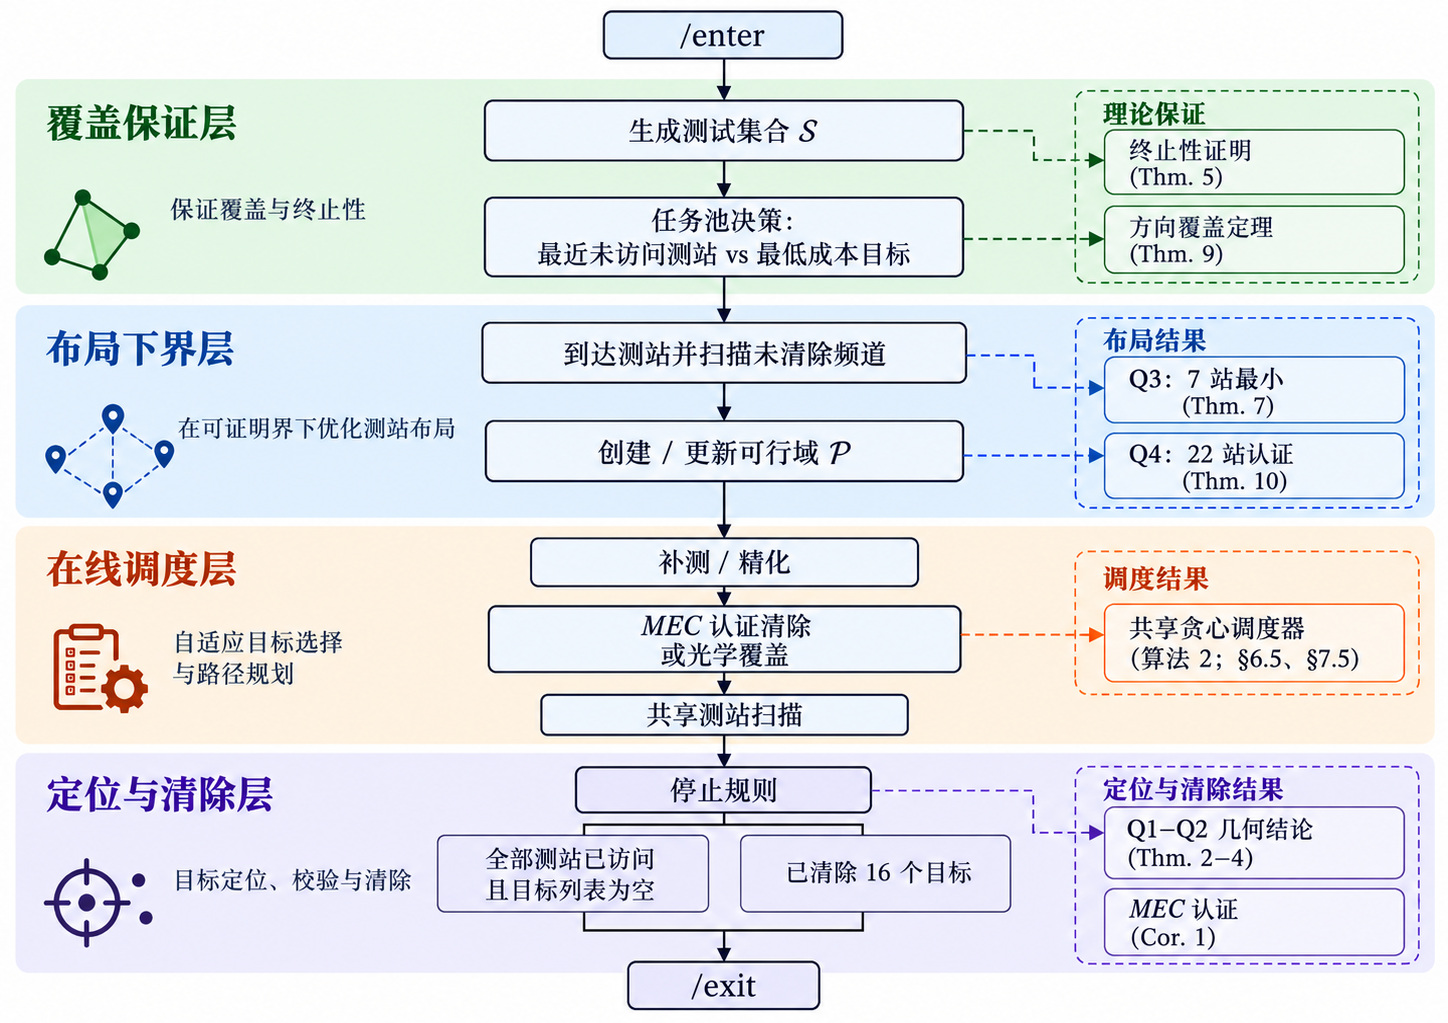
\includegraphics[width=\textwidth]{figures/fig-framework.png}
  \caption{总体求解框架：覆盖保证、布局下界、在线调度与定位清除四层}\label{fig:framework}
\end{figure}

\begin{table}[!htbp]
  \caption{数学保证、代码实现与逐例验收的对应}\label{tab:proof-impl}\centering\small
  \begin{tabularx}{\textwidth}{@{}L L L@{}}
    \toprule[1.5pt]
    数学保证 & 代码实现 & 逐例验收 \\
    \midrule[1pt]
    终止性（\cref{thm:term3}） & 走遍所有覆盖测站后才允许退出 & 逐例核对清除数 $=$ 真实源数 \\
    方向覆盖（\cref{thm:hull}） & 运行时 $20\mmet$ 粗网格凸包检查 & $h=1\mmet$ 网格证书 $1018.68$ 万点全部通过 \\
    认证清除（\cref{cor:certify}） & 仅当 $\mecr\le r_c-10^{-6}$ 才在圆心清除 & 清除点到真源距离 $\le20\mmet$ \\
    包含性不变量（\cref{eq:invariant}） & 目标圆外切、圆盘排除取凸包外近似 & 每时刻可行域与包围圆均含真源 \\
    \bottomrule[1.5pt]
  \end{tabularx}
\end{table}

\begin{table}[!htbp]
  \caption{在线决策流程的判定与动作}\label{tab:decision}\centering\small
  \begin{tabularx}{\textwidth}{@{}l L L@{}}
    \toprule[1.5pt]
    状态 & 判断条件 & 后续动作 \\
    \midrule[1pt]
    首测成功 & 返回 \texttt{direction} & 由方位约束建立可行域，进入定位 \\
    首测无信号 & 全向源返回 \texttt{no\_signal} & 以圆盘排除该站邻域；定向源改用其他测站 \\
    观测不足 & 可行域无界或仅 $1$ 条方位 & 走到第二测点或补测一次 \\
    可行域过大 & $\mecr>r_c$ & 圆心补测精化，仍不足则光学覆盖 \\
    认证通过 & $\mecr\le r_c-10^{-6}$ & 在最小包围圆圆心执行 \texttt{/clear} \\
    清除失败 & 接口拒绝或超时 & 限次重试，否则安全退出并留档 \\
    \bottomrule[1.5pt]
  \end{tabularx}
\end{table}

\subsection{四问的核心难点}

四问各自的核心困难可概括为：问题一要在有界角度误差下严格表示定位区域，并给出只依赖可行域的清除判据；问题二要让第二测点既保证收到信号又改善交会角，并说清两次测向的能力边界；问题三要在不知道源数与位置时证明“已全部发现”，并在保证全清下压缩固定成本；问题四中定向源使“距离覆盖”失效，需要新的方向覆盖条件。四问与四层的对应是：问题一提供定位证书（第\ref{sec:q1}节），问题二给出第二测点选择（第\ref{sec:q2}节），问题三完成全向源的覆盖与路径（第\ref{sec:q3}节），问题四给出定向源的方向覆盖与搜索布局（第\ref{sec:q4}节）。

\subsection{四个问题之间的关系}

需要强调，第三、四问是部分可观测的在线搜索控制问题：在走完所有测站之前，算法不知道还有几个源、在哪里，因此必须先回答“未发现源可能存在于哪些区域”和“何时可以安全结束”，才能借鉴路径优化的思想。

\paragraph{核心贡献.} 全文的主要贡献可凝练为四点：\textbf{其一}，建立“发现—定位—清除”的全覆盖保证框架，把终止条件建立在连续域几何覆盖上；\textbf{其二}，证明七站布局达到距离覆盖的理论下界（$6$ 站不可能）；\textbf{其三}，用凸包充要条件刻画定向源的方向覆盖，并给出 $22$ 站的连续域证书；\textbf{其四}，由时间构成诊断认定固定成本主导，据此把优化落到测站布局上。